\chapter{Tutorial}
	\par Insira aqui a introdução!!!
	
	\lipsum[1-5]
	
	
	
	\chapter{Algumas notas sobre bibliografia}
	
	
	\par O arquivo \textit{referencias.bib} é o nome padrão das referências para este modelo. Para alterá-lo modifique o argumento entre chaves na definição de bibliografia.
	
	
	\section{Modelos de citação}
	\par No arquivo modelo de referências, também existem alguns exemplos de diferentes classes de citações. Todas elas podem ser usadas com o \textit{$\backslash$cite$\{$label$\}$} ou \textit{$\backslash$citeonline$\{$label$\}$}, dependendo da forma de citação\footnote{Este é um teste de nota de rodapé}.
	
	\par Além disso, pode-se incluir obras na bibliografia que nortearam o trabalho mesmo que elas não apareçam diretamente no texto, utilizando o comando \textit{$\backslash$nocite$\{$label$\}$}. Além disso, pode-se citar vários trabalhos em conjunto, por exemplo:
	
	\begin{center}\rule{0.5\textwidth}{1pt}\\$\backslash cite\{label1,label2,label3,...\}$\end{center}
	
	\begin{verbatim}
		Os ventos do norte não movem moinhos \cite{tcc:mintegui2014, 
			diss:anabor2004, tese:anabor2008, livro:halliday28ed, 
			livro:fedorova:v1, site:amsglo:fog}.
	\end{verbatim}
	
	\par Os ventos do norte\footnote{Este é um teste de nota de rodapé} não movem moinhos \cite{tcc:mintegui2014,diss:anabor2004,tese:anabor2008,livro:halliday28ed,livro:fedorova:v1,site:amsglo:fog}.
	
	\begin{center}\rule{0.5\textwidth}{1pt}\\$\backslash citeonline\{label1,label2,label3,...\}$\end{center}
	
	\begin{verbatim}
		Segundo \citeonline{cap:livro:djuric1994, livro:aris1989, 
			livro:cotton1989, cap:livro:wyngaard1981, livro:fedorova:v1, 
			artigo:fujita1981,puhalesBLT2010,artigo:janjic2002,
			cbmet:anabor2012,site:wrfhome}, os ventos do norte não movem moinhos.
	\end{verbatim}
	
	\par Segundo \citeonline{cap:livro:djuric1994, livro:aris1989, livro:cotton1989, cap:livro:wyngaard1981, livro:fedorova:v1, artigo:fujita1981,puhalesBLT2010,artigo:janjic2002,cbmet:anabor2012,site:wrfhome}, os ventos\footnote{Este é um teste de nota de rodapé} do norte não movem moinhos.
	\begin{center}\rule{0.5\textwidth}{1pt}\end{center}   
	\par OBS: Trabalhos com mais de três autores aparecerão com a abreviatura ``et al'' no corpo do texto, porém todos os nomes da bibliografia (norma da UFSM que é definida nas opões do abntcite nas definições do arquivo). 
	
	\subsection{O comando \textit{apud}}
	
	\par A citação \textit{apud} ocorre quando você cita algum autor através de outra obra, sem ter consultado-a propriamente. Neste caso a citação é feita da seguinte forma:
	\begin{center}
		\rule{0.5\textwidth}{1pt}\\
		$\backslash apud\{material\_citado\_no\_material\_lido\}\{material\_lido\}$ \\
	\end{center}
	\begin{verbatim}
		Sobre a circulação geral da atmosfera pode-se dizer que os ventos do norte
		não movem moinhos \apud{apud:richardson1922}{livro:monin:v1}.
	\end{verbatim}
	
	Sobre a circulação geral da atmosfera pode-se dizer que os ventos do nortenão movem moinhos \apud{apud:richardson1922}{livro:monin:v1}.
	\begin{center}\rule{0.5\textwidth}{1pt}\end{center}  
	\par Nesse caso, na bibliografia só constará a obra consultada e não aquele referenciada pela obra. Para que isso ocorra naturalmente, a obra consultada deve ser incluída normalmente no arquivo referencias.bib enquanto a obra referenciada indiretamente deve ser incluída com a opção \textit{@hidden}, conforme o modelo de referências\footnote{Isto é um teste de nota de rodapé}.
	
	\subsubsection{\textit{Apud on line}}
	
	
	\par O \textit{apudonline} se aplica da mesma maneira que o \textit{apud} descrito anteriormente. O termo \textit{on line} é alusivo ao \textit{$\backslash$citeonline$\{$label$\}$} definido no abntex. Nesse caso a citação é feita da seguinte forma:
	\begin{center}
		\rule{0.5\textwidth}{1pt}
		$\backslash apudonline\{material\_citado\_no\_material\_lido\}\{material\_lido\}$ \\
	\end{center}
	
	\begin{verbatim}
		Segundo \apudonline{apud:richardson1922}{livro:monin:v1}, os ventos do
		norte não movem moinhos.
	\end{verbatim}
	
	Segundo \apudonline{apud:richardson1922}{livro:monin:v1}, os ventos do norte não movem moinhos.
	
	\paragraph{Teste de seção quinária}
	
	\par Texto texto texto.
	
	
	\chapter{Tabelas, figuras, quadros, ilustrações e gráficos}
	
	\par Na MDT da UFSM há uma clara diferença entre tabelas e quadros, quanto a sua apresentação. Aqui, para inserir tabelas usa-se o ambiente tradicionalmente definido \textit{table}. A partir deste modelo simples:
	
	\begin{verbatim}
		\begin{table}[ht]
			\centering
			\caption{Modelo de tabela para MDT-UFSM.}
			\begin{tabular}{ c c c }
				\hline
				Abacate & Banana & Canela \\
				\hline
				21 & 34 & 56 \\
				-3 & 245 & 23 \\
				-25 & -0,57 & 2 \\
				\hline
			\end{tabular}
			\fonte{Adaptado de \citeonline{livro:halliday28ed}.}
		\end{table}
	\end{verbatim}
	
	\noindent resulta:
	
	\begin{table}[ht]
		\centering
		\caption{Modelo de tabela para MDT-UFSM.}
		\begin{tabular}{ c c c }
			\hline
			Abacate & Banana & Canela \\
			\hline
			21 & 34 & 56 \\
			-3 & 245 & 23 \\
			-25 & -0,57 & 2 \\
			\hline
		\end{tabular}
		\fonte{Adaptado de \citeonline{livro:halliday28ed}.}
	\end{table}
	
	\par Note que, adicionalmente, foi definido um comando novo: ``fonte''. Ele serve para indicar a fonte da tabela quando necessário, mas também pode ser usado em outros ambientes.
	
	\par Para inserir quadros foi criado um novo ambiente: ``quadro''. O ambiente ``quadro'' deve ser usado de forma semelhante a tabela, como o ambiente tabular. Contudo, neste caso, as linhas verticais e horizontais estão sempre presentes. Um exemplo simples é o seguinte: 
	
	
	\begin{verbatim}
		\begin{quadro}
			\caption{Modelo de quadro para MTD-UFSM.}
			\centering
			\begin{tabular}{| c |c |c }
				\hline
				Abacate & Banana & Canela \\
				\hline
				21 & 34 & 56 \\
				\hline
				-3 & 245 & 23 \\
				\hline
				-25 & -0,57 & 2 \\
				\hline
			\end{tabular}
			\fonte{Adaptado de \citeonline{livro:halliday28ed}.}
		\end{quadro}
	\end{verbatim}
	
	\noindent resultando:
	
	\begin{quadro}
		\caption{Modelo de quadro para MTD-UFSM.}
		\centering
		\begin{tabular}{| c |c |c |}
			\hline
			Abacate & Banana & Canela \\
			\hline
			21 & 34 & 56 \\
			\hline
			-3 & 245 & 23 \\
			\hline
			-25 & -0,57 & 2 \\
			\hline
		\end{tabular}
		\fonte{Adaptado de \citeonline{livro:halliday28ed}.}
	\end{quadro}
	
	
	\noindent Assim como para as tabelas, já está definida uma lista de quadros. Além disso, o comando ``fonte'' também pode ser usado aqui se necessário. Vale lembrar que, na MDT-UFSM, as legendas para figuras, tabelas, quadros, ilustrações e gráficos devem ser inseridas no topo da(o) mesma(o). A fonte sempre embaixo.
	
	\par As figuras devem ser inseridas com o ambiente padrão: \textit{figure}. Veja um exemplo simples:
	
	\begin{verbatim}
		\begin{figure}[ht]
			\caption{\label{exepretex}Sequência dos elementros pré-testuais da MDT-UFSM.}
			\centering
			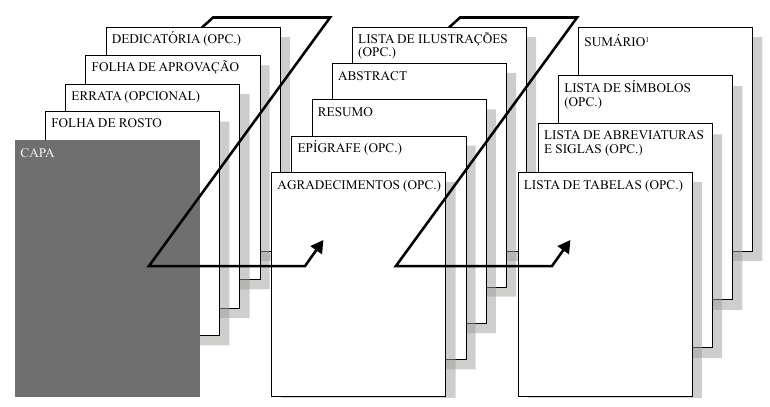
\includegraphics[width=0.6\textwidth]{figuras/pretextuais.png}
			\fonte{Adaptado de \citeonline{man:MDTUFSM2015}.}
		\end{figure}
	\end{verbatim}
	
	\begin{figure}[ht]
		\caption{\label{exepretex}Sequência dos elementros pré-testuais da MDT-UFSM.}
		\centering
		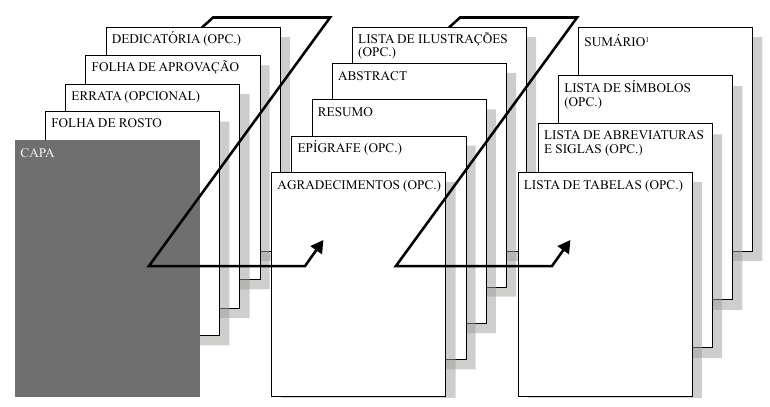
\includegraphics[width=0.6\textwidth]{figuras/pretextuais.png}
		\fonte{Adaptado de \citeonline{man:MDTUFSM2015}.}
	\end{figure}
	
	\par Para inserir ilustrações e gráficos, foram criados novos ambientes: ``ilustracao'' e ``grafico''. Estes ambientes são semelhantes ao ambiente ``figure'', porém geram sua própria lista. A seguir, exemplos da utilização nos novos ambientes.
	
	\begin{verbatim}
		\begin{ilustracao}[ht]
			\caption{\label{exepretex1}Sequência dos elementros pré-testuais da MDT-UFSM}
			\centering
			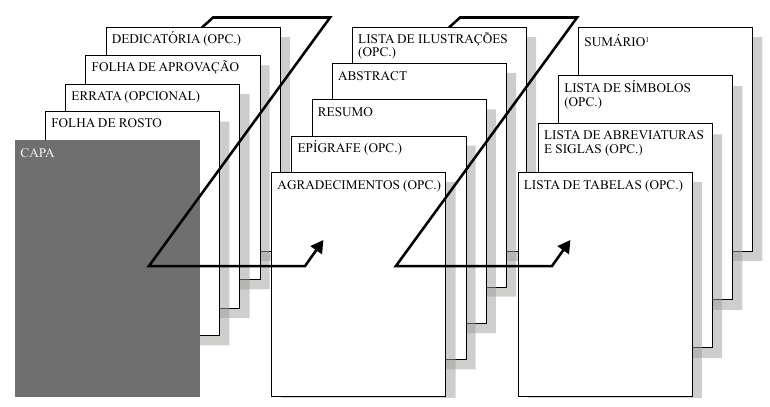
\includegraphics[width=0.6\textwidth]{figuras/pretextuais.png}
			\fonte{Adaptado de \citeonline{man:MDTUFSM2015}.}
		\end{ilustracao}
	\end{verbatim}
	
	\begin{ilustracao}[ht]
		\caption{\label{exepretex1}Sequência dos elementros pré-testuais da MDT-UFSM.}
		\centering
		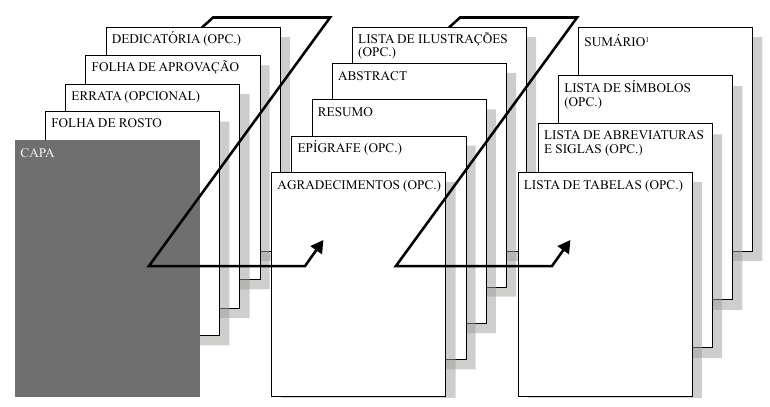
\includegraphics[width=0.6\textwidth]{figuras/pretextuais.png}
		\fonte{Adaptado de \citeonline{man:MDTUFSM2015}.}
	\end{ilustracao}
	
	
	\begin{verbatim}
		\begin{grafico}[ht]
			\centering
			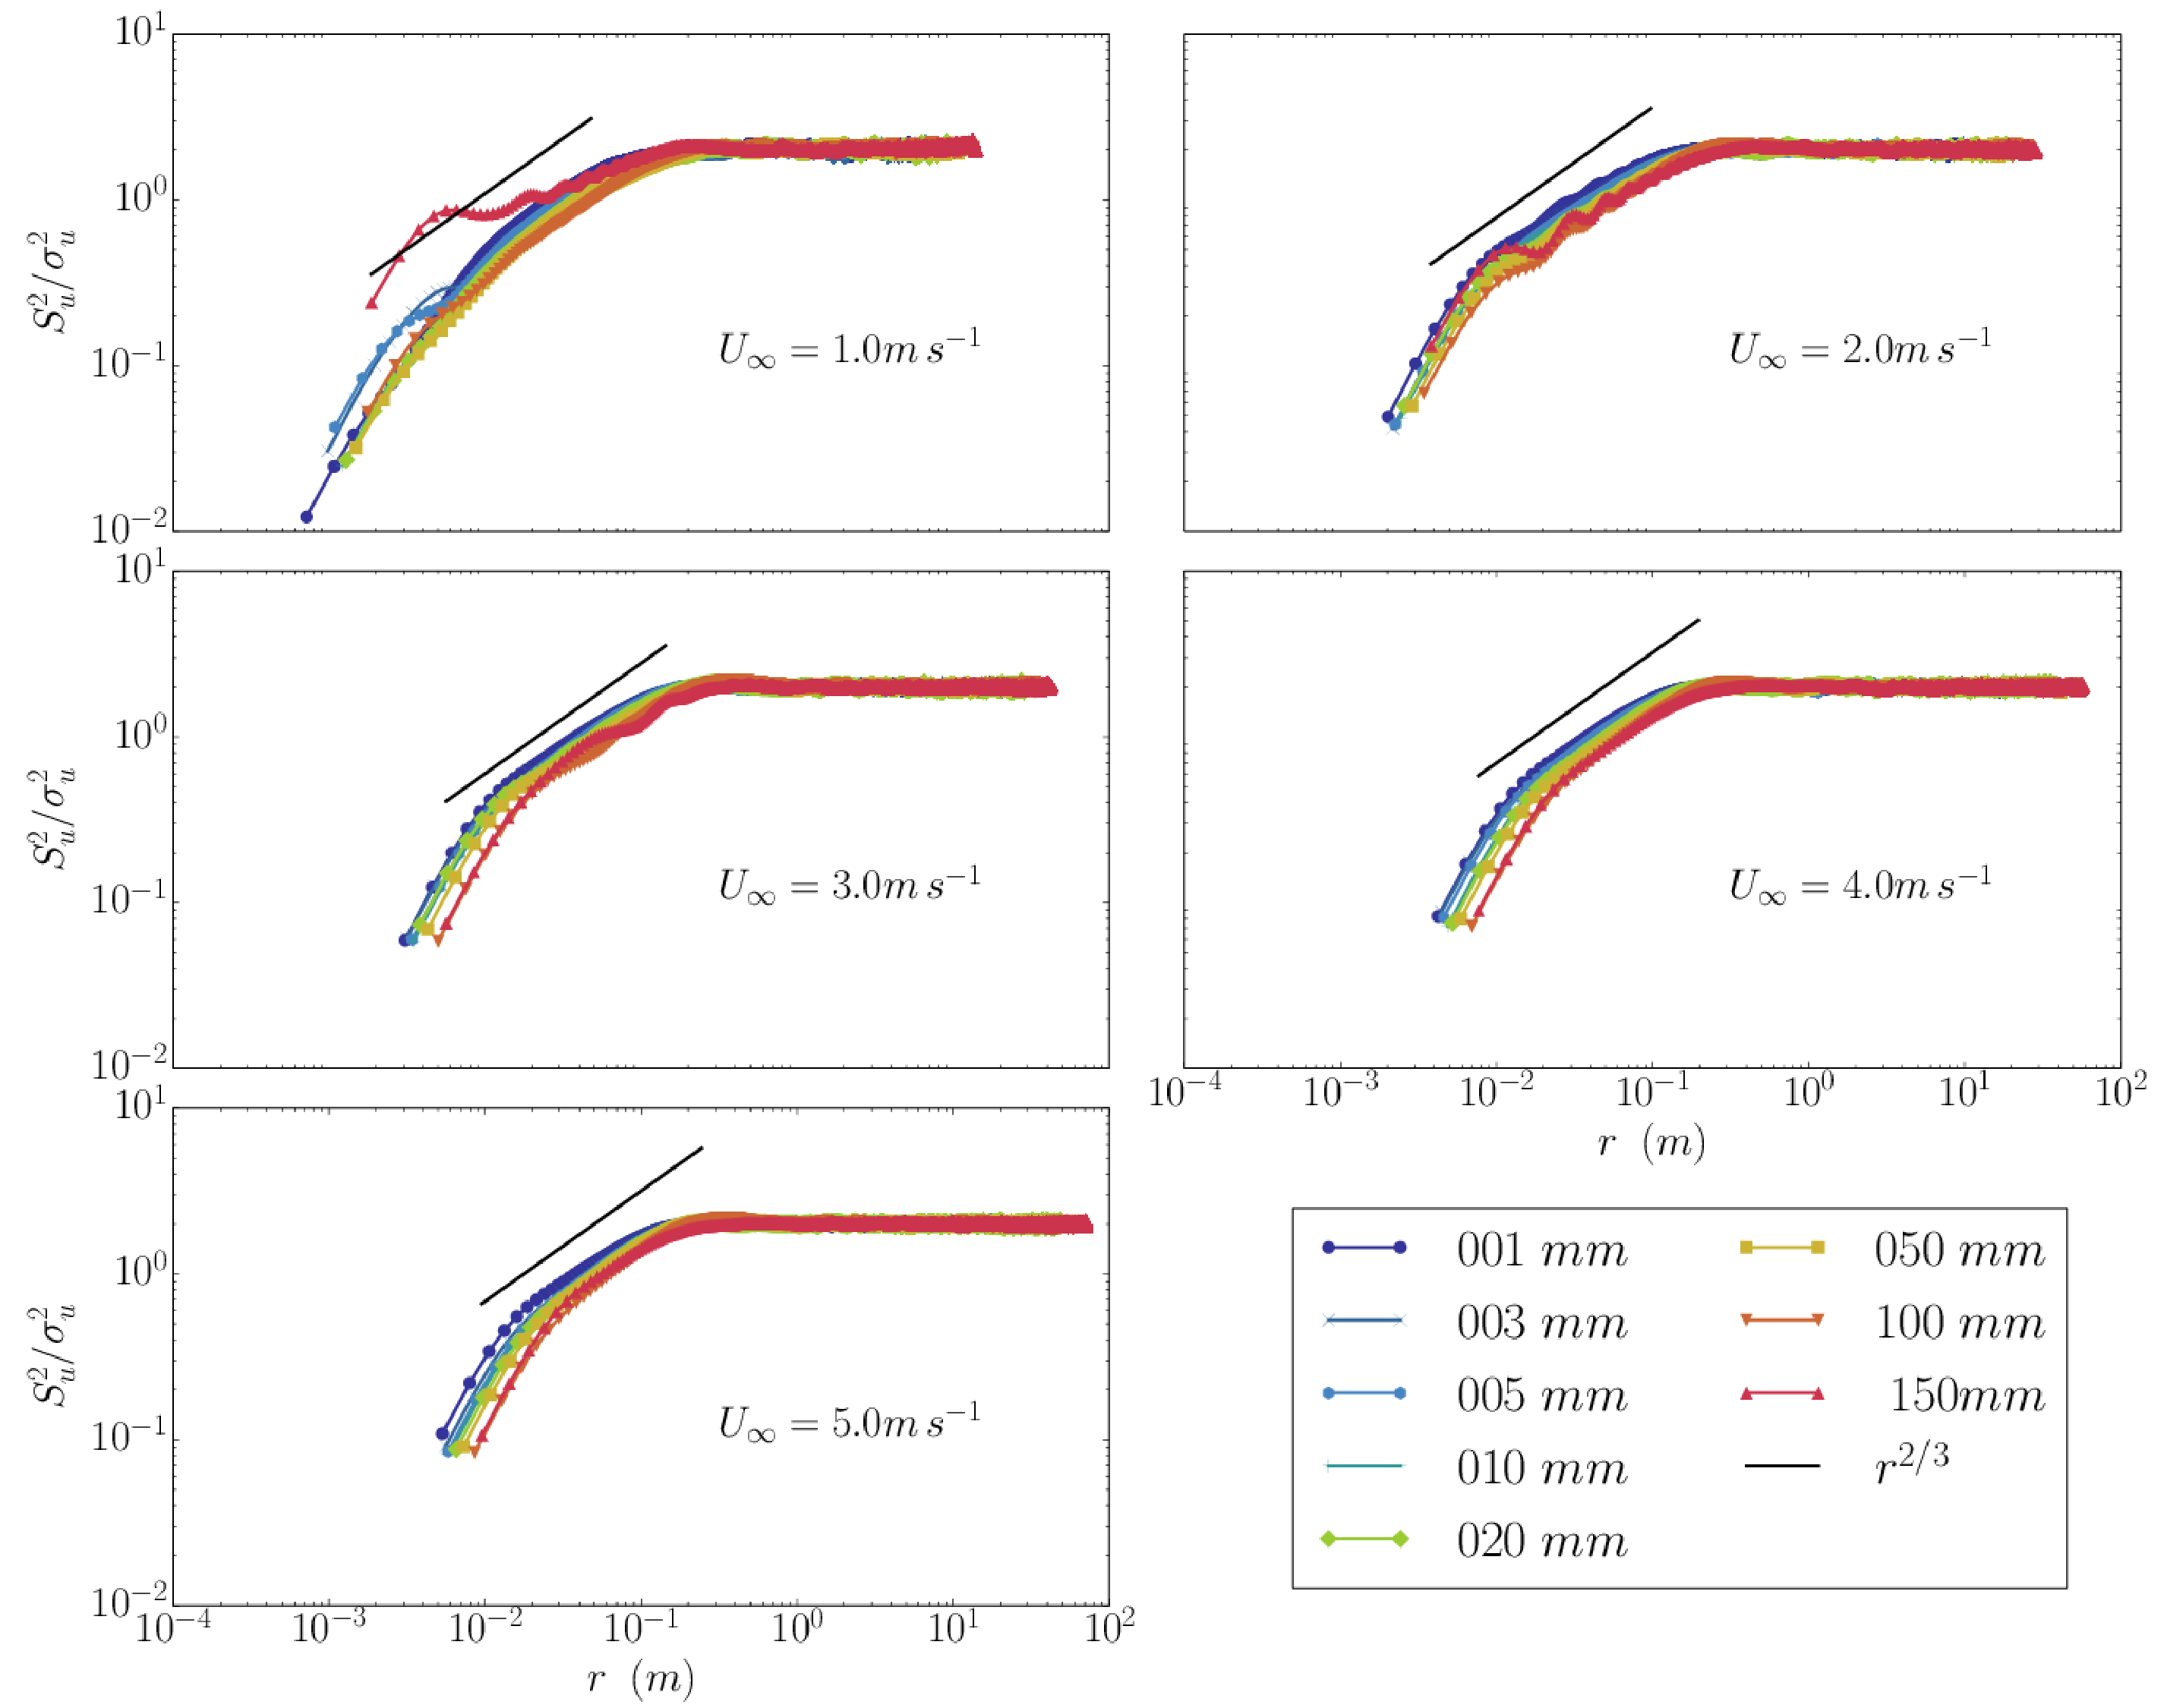
\includegraphics[width=0.6\textwidth]{figuras/estrutura_com.pdf}
			\caption{\label{exepretex3} Um exemplo de utilização do ambiente ``grafico''.}
			\fonte{Próprio autor.}
		\end{grafico}
	\end{verbatim}
	
	\begin{grafico}[ht]
		\caption{\label{exepretex3}Um exemplo de utilização do ambiente ``grafico''.}
		\centering
		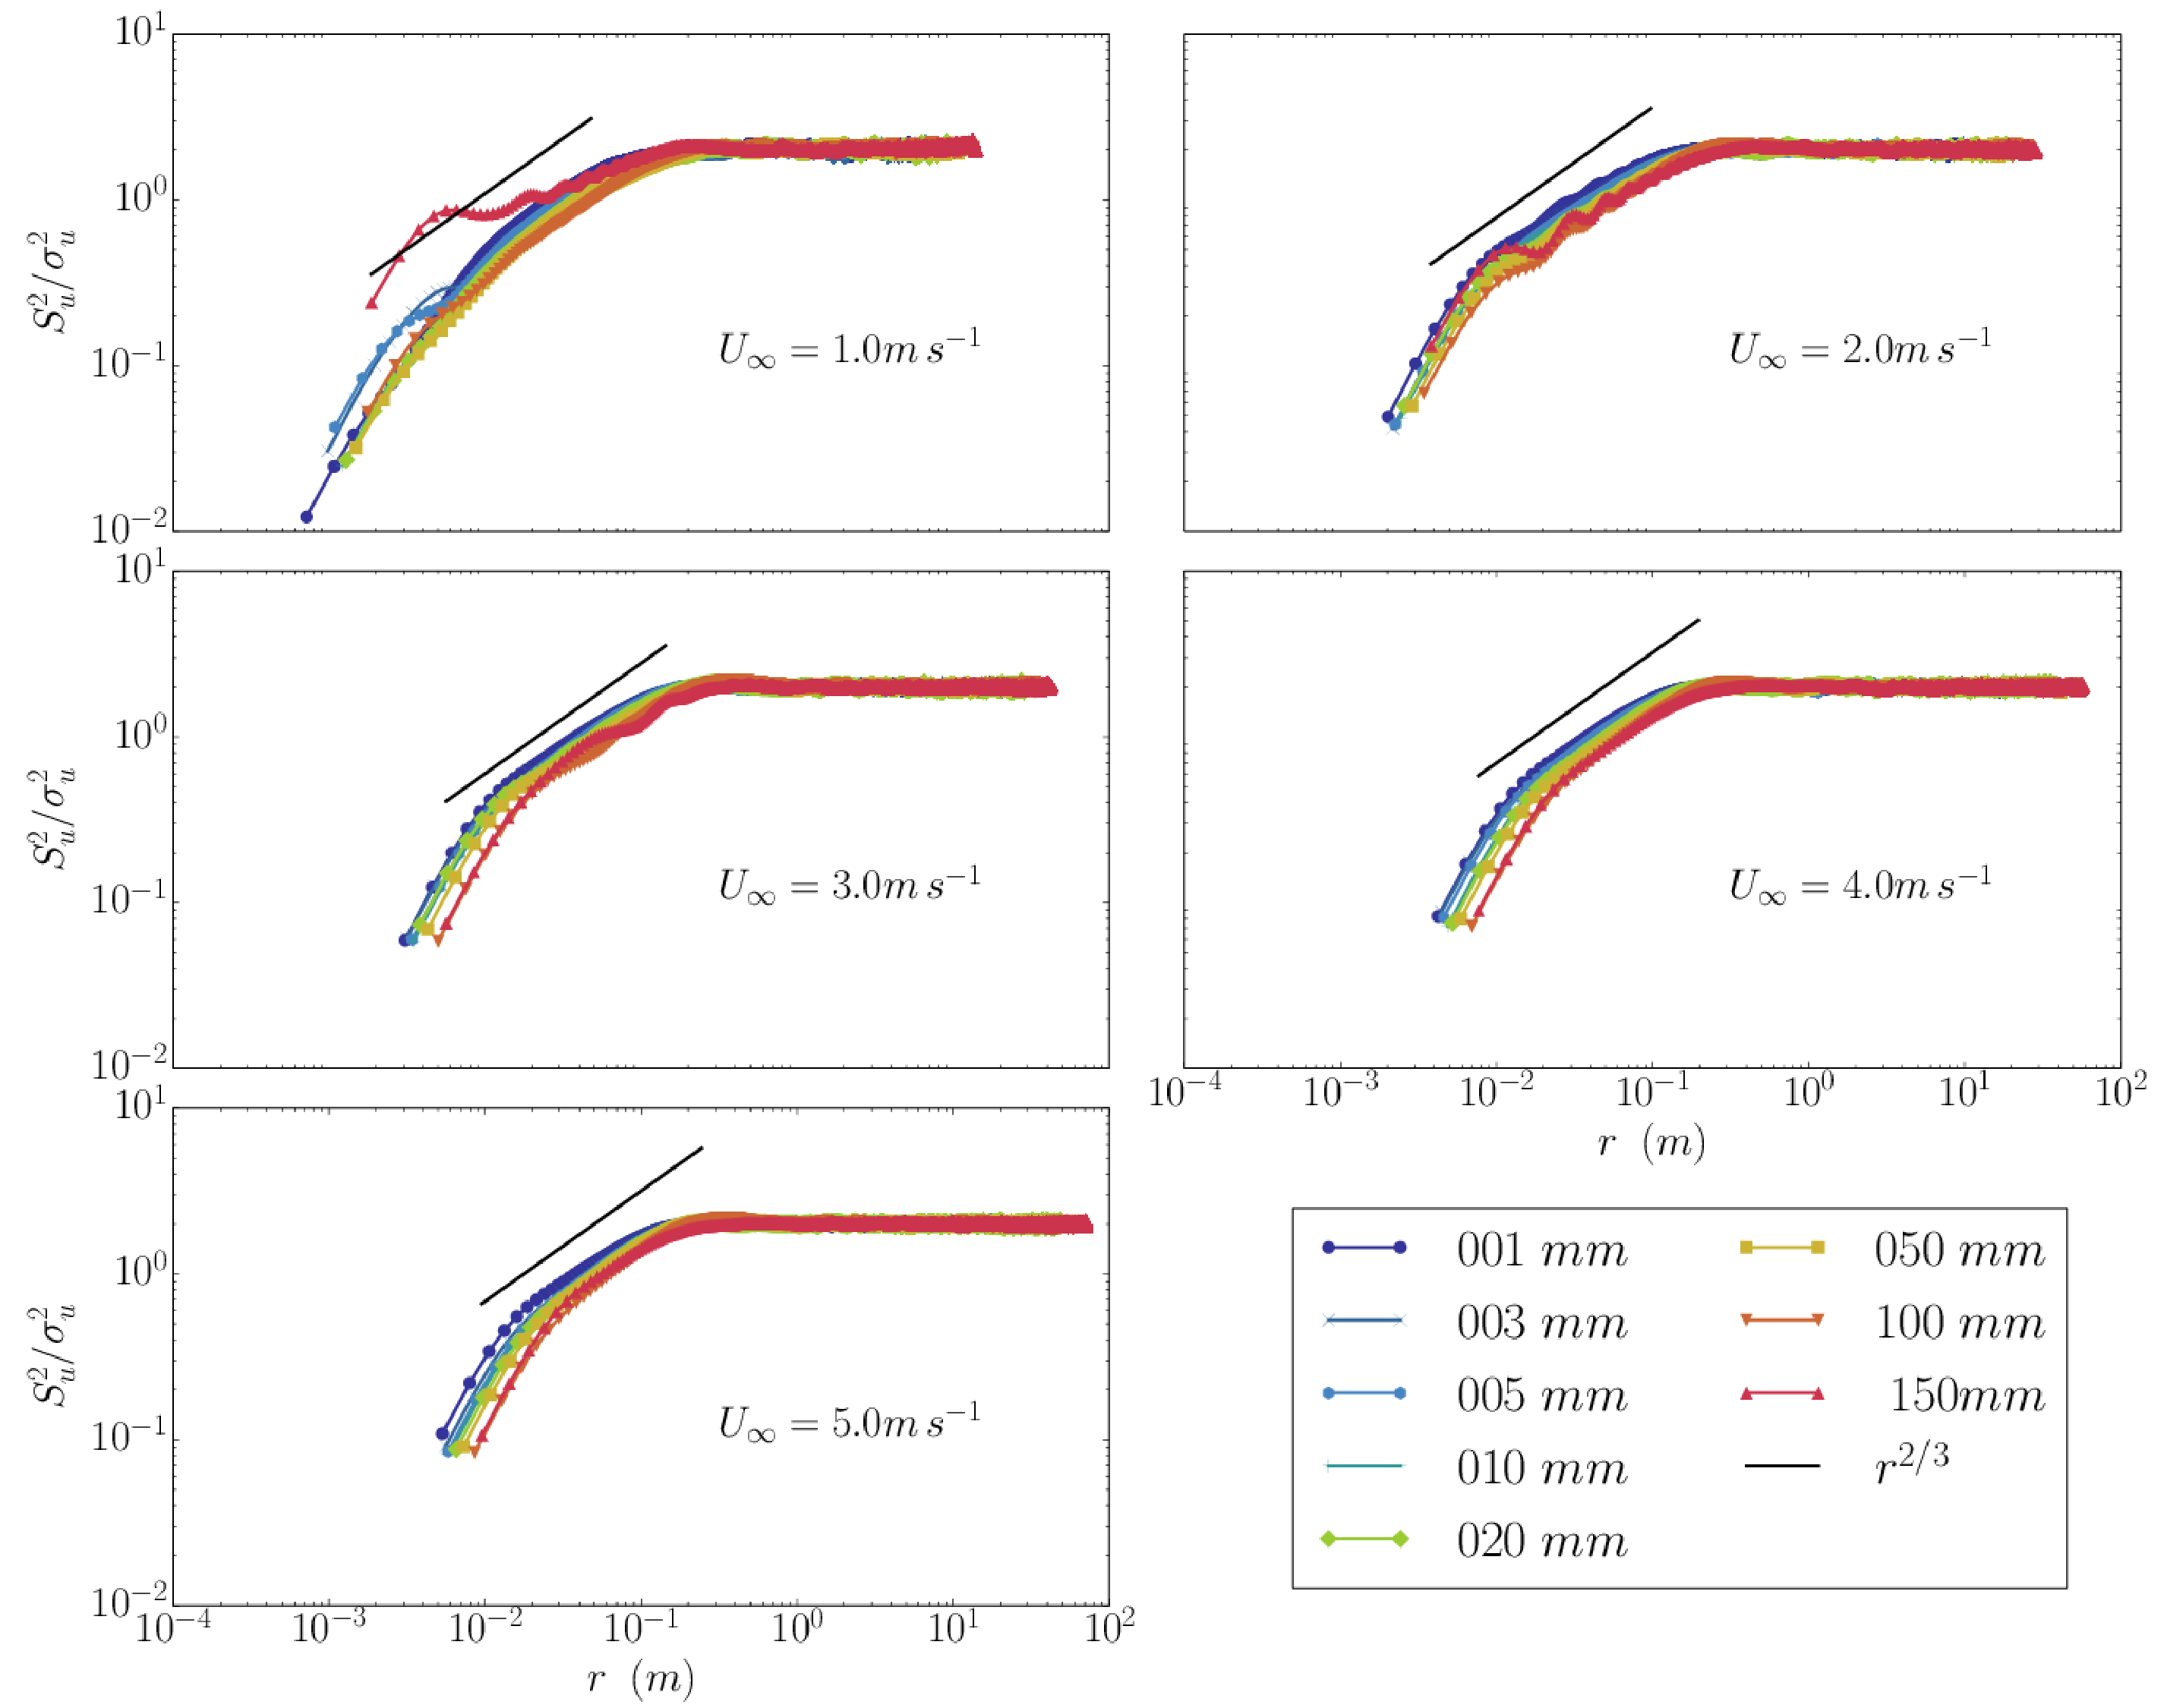
\includegraphics[width=0.6\textwidth]{figuras/estrutura_com.pdf}
		\fonte{Próprio autor.}
	\end{grafico}
	
	
	
	